%%
%% getstart.tex -- Flight Gear documentation: The FlightGear Manual
%% Chapter file
%%
%% Written by Michael Basler, started September 1998.
%%
%% Copyright (C) 2002 Michael Basler
%%
%%
%% This program is free software; you can redistribute it and/or
%% modify it under the terms of the GNU General Public License as
%% published by the Free Software Foundation; either version 2 of the
%% License, or (at your option) any later version.
%%
%% This program is distributed in the hope that it will be useful, but
%% WITHOUT ANY WARRANTY; without even the implied warranty of
%% MERCHANTABILITY or FITNESS FOR A PARTICULAR PURPOSE.  See the GNU
%% General Public License for more details.
%%
%% You should have received a copy of the GNU General Public License
%% along with this program; if not, write to the Free Software
%% Foundation, Inc., 675 Mass Ave, Cambridge, MA 02139, USA.
%%
%% $Id: free.tex,v 0.6 2002/09/09 michael
%% (Log is kept at end of this file)

%%%%%%%%%%%%%%%%%%%%%%%%%%%%%%%%%%%%%%%%%%%%%%%%%%%%%%%%%%%%%%%%%%%%%%%%%%%%%%%%%%%%%%%%%%%%%%%
\chapter{Want to have a free flight? Take {\FlightGear{}}!\label{free}}
%%%%%%%%%%%%%%%%%%%%%%%%%%%%%%%%%%%%%%%%%%%%%%%%%%%%%%%%%%%%%%%%%%%%%%%%%%%%%%%%%%%%%%%%%%%%%%%

%%%%%%%%%%%%%%%%%%%%%%%%%%%%%%%%%%%%%%%%%%%%%%%%%%%%%%%%%%%%%%%%%%%%%%%%%%%%%%%%%%%%%%%%%%%%%%%
\section{Yet Another Flight Simulator?}
%%%%%%%%%%%%%%%%%%%%%%%%%%%%%%%%%%%%%%%%%%%%%%%%%%%%%%%%%%%%%%%%%%%%%%%%%%%%%%%%%%%%%%%%%%%%%%%
\markboth{\thechapter.\hspace*{1mm} WANT TO HAVE A FREE FLIGHT?}{\thesection\hspace*{1mm}
YET ANOTHER FLIGHT SIMULATOR?}

Did you ever want to fly a plane yourself, but lacked the money or ability to do so? Are
you a real pilot looking to improve your skills without having to take off? Do you want
to try some dangerous maneuvers without risking your life? Or do you just want to have
fun with a more serious game without any violence? If any of these questions apply
to you, PC flight simulators are just for you.

You may already have some experience using \Index{Microsoft}'s {\copyright} Flight Simulator
or any other of the commercially available PC flight simulators. As the
price tag of those is usually within the {\$}50 range, buying one of them should not be a
serious problem given that running any serious PC flight simulator requires PC hardware
within the {\$}1500 range, despite dropping prices.

With so many commercially available flight simulators, why would we spend
thousands of hours of programming and design work to build a free flight
simulator?  Well, there are many reasons, but here are the major ones:

\begin{itemize}
 \item All of the commercial simulators have a serious drawback: they are made
 by a small group of developers defining their properties according to what
 is important to them and providing limited interfaces to end users.  Anyone
 who has ever tried to contact a commercial developer would agree that getting
 your voice heard in that environment is a major challenge.  In contrast,
 \FlightGear{} is designed by the people and for the people with everything
 out in the open.

 \item Commercial simulators are usually a compromise of features and
 usability.  Most commercial developers want to be able to serve a broad
 segment of the population, including serious pilots, beginners, and even
 casual gamers.
 In reality the result is always a compromise due to deadlines and
 funding.  As \FlightGear{} is free and open, there is no need for such
 a compromise.  We have no publisher breathing down our necks, and
 we're all volunteers that make our own deadlines.  We are also at
 liberty to support markets that no commercial developer would consider
 viable, like the scientific research community.
 \item Due to their closed-source nature, commercial simulators keep developers
 with excellent ideas and skills from contributing to the products.  With
 \FlightGear{}, developers of all skill levels and ideas have the potential
 to make a huge impact on the project.  Contributing to a project as large
 and complex as \FlightGear{} is very rewarding and provides the developers
 with a great deal of pride in knowing that we are shaping the future of a
 great simulator.
 \item Beyond everything else, it's just plain fun!  I suppose you could
 compare us to real pilots that build kit-planes or scratch-builts.  Sure,
 we can go out a buy a pre-built aircraft, but there's just something special
 about building one yourself.
\end{itemize}

The points mentioned above form the basis of why we created \FlightGear{}.
With those motivations in mind, we have set out to create a high-quality
flight simulator that aims to be a civilian,\index{Flight simulator!civilian}
multi-platform,\index{Flight simulator!multi-platform} open,\index{Flight simulator!open}
user-supported,\index{Flight simulator!user-sported} and user-extensible\index{Flight
simulator!user-extensible} platform.  Let us take a closer look at each of these
characteristics:

\begin{itemize}
 \item \textbf{Civilian:}\index{Flight simulator!civilian} The project is primarily aimed
 at civilian flight simulation.  It should be appropriate for simulating general aviation
 as well as civilian aircraft.  Our long-term goal is to have \FlightGear{} FAA-approved as
 a flight training device.  To the disappointment of some users, it is currently not a
 combat simulator; however, these features are not explicitly excluded.  We just have
 not had a developer that was seriously interested in systems necessary for combat
 simulation.

 \item\textbf{Multi-platform:}\index{Flight simulator!multi-platform} The
 developers are attempting to keep the code as platform-independent as possible. This
 is based on their observation that people interested in flight simulations run quite a
 variety of computer hardware and operating systems. The present code supports the
 following \Index{Operating Systems}:
  \begin{itemize}
  \item\Index{Linux} (any distribution and platform),
  \item\Index{Windows NT/2000/XP} (Intel/AMD platform),
  \item\Index{Windows 95/98/ME},
  \item\Index{BSD UNIX},
  \item\Index{Sun-OS},
  \item{Mac OS X}
  \end{itemize}

At present, there is no other known flight simulator -- commercial or free
-- supporting such a broad range of platforms.

  \item\textbf{Open:}\index{Flight simulator!open} The project is not restricted to a
  static or elite cadre of developers. Anyone who feels they are able to contribute
  is most welcome.  The code (including documentation) is copyrighted under the
  terms of the \Index{GNU General Public License} (\Index{GPL}).

  The \Index{GPL} is often misunderstood. In simple terms it states that you
  can copy and freely distribute the program(s) so licensed.  You can modify
  them if you like and even charge as much money as want to for the
  distribution of the modified or original program.  However, when
  distributing the software you must make it available to the recipients in
  source code as well and it must retain the original copyrights.
  In short:
\medskip

\centerline{\textit{''You can do anything with the software except make it non-free''}.}

The full text of the \Index{GPL} can be obtained from the \FlightGear{} source code or from
 \medskip

\web{http://www.gnu.org/copyleft/gpl.html}.
 \medskip

\item\textbf{User-supported and user-extensible:}\index{Flight simulator!user-supported}
  \index{Flight simulator!user-extensible} Unlike most commercial simulators,
  \FlightGear{}'s scenery and aircraft formats, internal variables, APIs, and everything
  else are user accessible and documented from the beginning. Even without any explicit
  development \Index{documentation} (which naturally has to be written at some point),
  one can always go to the \Index{source code} to see how something works. It is the
  goal of the developers to build a basic engine to which scenery designers, panel
  engineers, maybe adventure or ATC routine writers, sound artists, and others can build
  upon. It is our hope that the project, including the developers and end users, will
  benefit from the creativity and ideas of the hundreds of talented ``simmers'' around
  the world.
\end{itemize}

  Without doubt, the success of the \Index{Linux} project, initiated by Linus
  Torvalds,\index{Torvalds, Linus} inspired several of the developers.
  Not only has \Index{Linux} shown that distributed development of highly
  sophisticated software projects over the Internet is possible, it has also
  proven that such an effort can surpass the level of quality of competing
  commercial products.
\medskip

 \centerline{\fbox{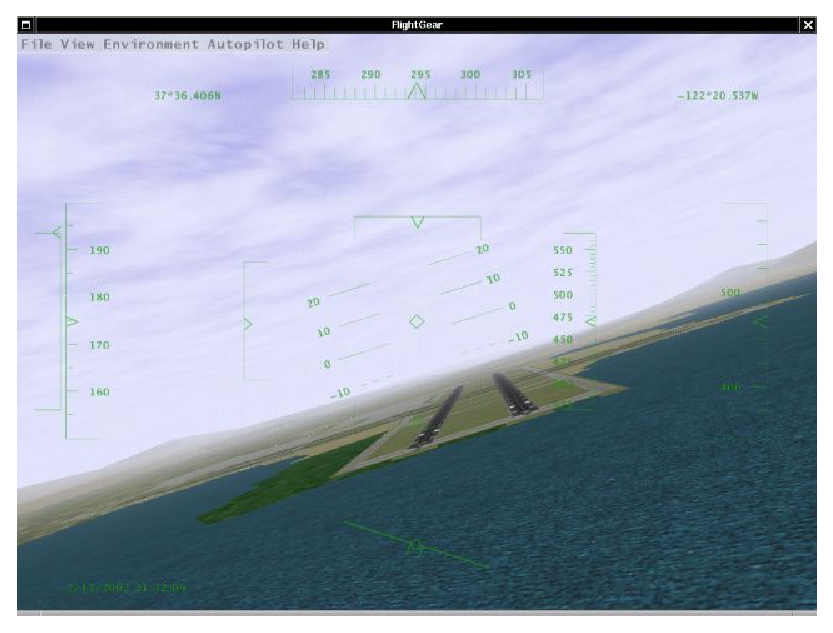
\includegraphics[clip,width=12.5cm]{KSFOapp}
}}

\smallskip
 \noindent
Fig.\,1: \FlightGear{} under UNIX: \textit{Bad approach to San Francisco International - by one of the authors of this manual\ldots}

%%%%%%%%%%%%%%%%%%%%%%%%%%%%%%%%%%%%%%%%%%%%%%%%%%%%%%%%%%%%%%%%%%%%%%%%%%%%%%%%%%%%%%%%%%%%%%%
\section{System Requirements}\index{system requirements}
%%%%%%%%%%%%%%%%%%%%%%%%%%%%%%%%%%%%%%%%%%%%%%%%%%%%%%%%%%%%%%%%%%%%%%%%%%%%%%%%%%%%%%%%%%%%%%%
In comparison to other recent flight simulators, the \Index{system requirements} for
\FlightGear{} are not extravagant. A medium speed AMD Athlon64 or Intel
P4, even a decent AMD Athlon/K7 or an Intel PIII should be sufficient
to handle \FlightGear{} pretty well, given you have a proper 3D \Index{graphics
card}.

One important prerequisite for running \FlightGear{} is a graphics card whose driver supports
\Index{OpenGL}. If you don't know what \Index{OpenGL} is, the overview given at the OpenGL website
\medskip

\web{http://www.opengl.org}
\medskip

\noindent
 says it best: ``Since its introduction in 1992, OpenGL has become the
industry's most widely used and supported 2-D and 3D graphics application programming
interface (API)...''.

\FlightGear{} does not run (and will never run) on a graphics board which only supports
\Index{Direct3D}. Contrary to OpenGL, Direct3D is a proprietary interface, being restricted to
the Windows operating system.

You may be able to run \FlightGear{} on a computer that features a 3D video card not
supporting hardware accelerated \Index{OpenGL} -- and even on systems without 3D
graphics hardware at all. However, the absence of hardware accelerated OpenGL support can bring even the fastest machine to its knees. The typical signal for missing hardware acceleration
are \Index{frame rate}s below 1 frame per second.

Any modern 3D graphics featuring \Index{OpenGL} support will do. For
\Index{Windows} video card drivers that support OpenGL, visit the home page of your video
card manufacturer. You should note that sometimes OpenGL drivers\index{OpenGL!drivers}
are provided by the manufacturers of the graphics chip instead of by the makers of the
board. If you are going to buy a graphics card for running \FlightGear{}, one based on a
AMD/ATI Radeon or NVIDIA GeForce with an absolute minimum of 64 MByte,
better 128 Mbyte might be a good choice.

To install the executable and basic scenery, you will need around 500 MB of free \Index{disk
space}. In case you want/have to compile the program yourself you will need about another
500 MB for the source code and for temporary files created during compilation. This does not
include the development environment, which will vary in size depending on the operating system
and environment being used.  Windows users can expect to need approximately 300 MB of additional
disk space for the development environment.  Linux and other UNIX machines should have most of
the development tools already installed, so there is likely to be little additional space
needed on those platforms.


For the \Index{sound effects}, any capable \Index{sound card} should suffice.
Due to its flexible design, \FlightGear{} supports a wide range of \Index{joysticks} and
\Index{yokes} as well as \Index{rudder pedals} under \Index{Linux} and \Index{Windows}. 
\FlightGear{} can also provide interfaces to full-motion flight chairs.

\FlightGear{} is being developed primarily under \Index{Linux}, a free UNIX clone
(together with lots of GNU utilities) developed cooperatively over the Internet in much
the same spirit as \FlightGear{} itself. \FlightGear{} also runs and is partly developed
under several flavors of \Index{Windows}. Building \FlightGear{} is also possible on a Mac OS X
and several different UNIX/X11 workstations. Given you have a proper \Index{compiler} installed,
\FlightGear{} can be built under all of these platforms. The primary compiler for all platforms is
the free \Index{GNU C++} compiler (the \Index{Cygnus} \Index{Cygwin} compiler under Win32).

If you want to run \FlightGear under Mac OS X, you need to have Mac OS X 10.4 or higher. 
Minimum hardware requirement is either a Power PC G4 1.0GHz or an intel Mac, but We suggest 
you have MacBook Pro, intel iMac, Mac Pro, or Power Mac (Power PC G5) for comfortable flight.
 

%%%%%%%%%%%%%%%%%%%%%%%%%%%%%%%%%%%%%%%%%%%%%%%%%%%%%%%%%%%%%%%%%%%%%%%%%%%%%%%%%%%%%%%%%%%%%%%
\section{Choosing A Version}\index{FlightGear!versions}
%%%%%%%%%%%%%%%%%%%%%%%%%%%%%%%%%%%%%%%%%%%%%%%%%%%%%%%%%%%%%%%%%%%%%%%%%%%%%%%%%%%%%%%%%%%%%%%

Previously the \FlightGear{} source code existed in two branches, a
stable branch and a developmental branch.\index{branch,
stable}\index{branch, developmental} Even version numbers like 0.6,
0.8, and (someday hopefully) 1.0 refer to stable releases, while odd
numbers like 0.7, 0.9, and so on refer to developmental releases.
This policy has been obsoleted by practical reasons - mostly because
stable releases got out-ouf-date and behind in features very fast and
the so called development releases had been proven to be of comparable
stability.\label{branches}

You are invited to fetch the ``latest official release'' which the
pre-compiled binaries are based on.  It is available from
\medskip

\web{http://www.flightgear.org/Downloads/}
\medskip

If you really want to get the very latest and greatest (and, at times,
buggiest) code, you can use a tool called \Index{anonymous cvs}\index{cvs, anonymous}
to get the recent code. A detailed description of how to set this up for \FlightGear{}
can be found at
 \medskip

\web{http://www.flightgear.org/cvs.html}.
 \medskip

 \noindent
 Given that the recent developmental versions on the
 other hands may contain bugs (\ldots undocumented features), we recommend using the
 ``latest official (unstable) release'' for the average user. This is the latest version named at

 \web{http://www.flightgear.org/News/}.

%%%%%%%%%%%%%%%%%%%%%%%%%%%%%%%%%%%%%%%%%%%%%%%%%%%%%%%%%%%%%%%%%%%%%%%%%%%%%%%%%%%%%%%%%%%%%%%
\section{Flight Dynamics Models\label{flightmodels}}\index{flight dynamics model}\index{flight model}
%%%%%%%%%%%%%%%%%%%%%%%%%%%%%%%%%%%%%%%%%%%%%%%%%%%%%%%%%%%%%%%%%%%%%%%%%%%%%%%%%%%%%%%%%%%%%%%
Historically, \FlightGear{} has been based on a flight model it inherited (together
with the Navion airplane) from LaRCsim. As this had several limitations (most importantly,
many characteristics were hard wired in contrast to using configuration files), there were
several attempts to develop or include alternative \Index{flightmodels}. As a result,
\FlightGear{} supports several different flight models, to be chosen from at runtime.

The most important one is the JSB flight model developed by Jon Berndt. Actually, the JSB
flight model is part of a stand-alone project called \JSBSim, having its home at
 \medskip

\web{http://jsbsim.sourceforge.net/}.
 \medskip

 \noindent
Concerning airplanes, the JSB flight model at present provides support for a
\Index{Cessna 172}, a \Index{Cessna 182}, a \Index{Cessna 310}, and for an experimental plane
called \Index{X15}. Jon and his group are gearing towards a very accurate flight model, and the
JSB model has become \FlightGear{}'s default flight model.

As an interesting alternative, Christian Mayer developed a flight model of a hot air
balloon. Moreover, Curt Olson integrated a special ``UFO'' slew mode, which
helps you to quickly fly from point A to point B.

Recently, Andrew Ross contributed another flight model called \YASim{}\index{YASim} for
\textit{Yet Another Simulator}. At present, it sports another \Index{Cessna 172}, a
\Index{Turbo 310}, a fairly good \Index{DC-3} model, along with a \Index{Boeing 747},
\Index{Harrier}, and \Index{A4}. \YASim{} takes a fundamentally different approach since it's
based on geometry information rather than aerodynamic coefficients. Where \JSBSim{} will be exact for every situation that is known and flight tested, but may have odd and/or unrealistic behavior outside normal flight, \YASim{} will be sensible and consistent in almost every flight situation, but is likely to differ in performance numbers.

As a further alternative, there is the \Index{UIUC flight model}, developed by a 
team at the University of Illinois at Urbana-Champaign.  This work was 
initially geared toward modeling aircraft in icing conditions\index{icing!modelling} together with a smart icing system to better enable pilots to fly safely in an icing 
encounter.  While this research continues, the project has expanded to 
include modeling ``nonlinear'' aerodynamics, which result in more realism 
in extreme attitudes, such as stall and high angle of attack flight.  Two 
good examples that illustrate this capability are the \Index{Airwave Xtreme 150} 
\Index{hang glider} and the 1903 \Index{Wright Flyer}.  For the hang glider, throttle can 
be used to fly to gliding altitude or Ctrl-U can be used to jump up in 
1000-ft increments.  Try your hand at the unstable Wright Flyer and don't 
stall the canard!  Considerable up elevator trim will be required for level 
flight.  In general, the aerodynamics are probably very close to the 
original Wright Flyer as they are partly based on experimental data taken 
on a replica tested recently at the NASA Ames Research Center.  Also 
included are two more models, a \Index{Beech 99} and \Index{Marchetti S-211} jet trainer, 
which are older generation UIUC/FGFS models and based on simpler ``linear'' 
aerodynamics.  More details of the UIUC flight model and a list of aircraft 
soon to be upgraded can be found on their website at
\medskip

\href{http://www.uiuc.edu/ph/www/m-selig/apasim.html}{http://www.uiuc.edu/ph/www/m-selig/apasim.html}
\medskip

It is even possible to drive FlightGear's scene display using an external
FDM\index{FDM!external} running on a different computer or via named
pipe\index{FDM!pipe} on the local machine -- although this might not be a
setup recommended to people just getting in touch with \FlightGear.


%%%%%%%%%%%%%%%%%%%%%%%%%%%%%%%%%%%%%%%%%%%%%%%%%%%%%%%%%%%%%%%%%%%%%%%%%%%%%%%%%%%%%%%%%%%%%%%
\section{About This Guide}
%%%%%%%%%%%%%%%%%%%%%%%%%%%%%%%%%%%%%%%%%%%%%%%%%%%%%%%%%%%%%%%%%%%%%%%%%%%%%%%%%%%%%%%%%%%%%%%
\markright{\thesection.\hspace*{1mm} ABOUT THIS GUIDE}

There is little, if any, material in this Guide that is presented here exclusively. You
could even say with Montaigne that we ``merely gathered here a big bunch of other men's
flowers, having furnished nothing of my own but the strip to hold them together''. Most
(but fortunately not all) of the information herein can also be obtained from the
\FlightGear{} web site\index{FlightGear Website} located at
\medskip

\web{http://www.flightgear.org/}
\medskip

Please, keep in mind that there are several mirrors of the \FlightGear{} web sites, all
of which are linked to from the \FlightGear{} homepage listed above.
You may prefer to download \FlightGear{} from a mirror closer to you than from the
main site.

\textit{The \FlightGear{} Manual} is intended to be a first step
towards a complete \FlightGear{} documentation\index{FlightGear
documentation}. The target audience is the end-user who is not
interested in the internal workings of \Index{OpenGL} or in building
his or her own scenery. It is our hope that someday there will be an
accompanying \textit{\FlightGear{} Programmer's Guide}\index{FlightGear
Programmer's Guide} (which could be based on some of the documentation
found at
 \medskip

\web{http://www.flightgear.org/Docs});
 \medskip

 \noindent
a \textit{\FlightGear{} Scenery Design Guide},\index{FlightGear Scenery Design Guide}
describing the Scenery tools now packaged as \TerraGear{}; and a \textit{\FlightGear{}
Flight School}\index{FlightGear Flight School} package.
 \medskip

As a supplement, we recommend reading the \FlightGear{} FAQ to be found at

\web{http://www.flightgear.org/Docs/FlightGear-FAQ.html}

which has a lot of supplementary information that may not be included in this manual.

\textbf{We kindly ask you to help us refine this document by submitting corrections,
improvements, and suggestions. All users are invited to contribute
descriptions of alternative setups (graphics cards, operating systems
etc.). We will be more than happy to include those in future versions
of \textit{The FlightGear Manual} (of course not without giving credit
to the authors).}

While we intend to continually update this document, we may not be able to produce a
new version for every single release of {\FlightGear{}}.  To do so would require more
manpower than we have now, so please feel free to jump in and help out.  We hope to
produce documentation that measures up to the quality of \FlightGear{} itself.


%% Revision 0.00  1998/09/08  michael
%% Initial revision for version 0.53.
%% Revision 0.01  1998/09/20  michael
%% several extensions and corrections
%% revision 0.10  1998/10/01  michael
%% final proofreading for release
%% revision 0.11  1998/11/01  michael
%% minor corrections on platforms, satellite data, OpenGL
%% added Navion pic
%% revision 0.12  1999/03/07  michael
%% update on recent development
%% revision 0.20  1999/06/04  michael
%% updates on recent development, corrections of links
%% revision 0.3 2000/04/20 michael
%% Rewritten for version 0.7.2, many changes, added development since summer 1999,
%% development vs. stable version, split into SimGear/FlightGear/TerraGear
%% Proofread by Jon Berndt
%% revision 0.4 2001/05/12 michael
%% update on development during the last year, corrections on requirements,
%% new sections on different versions and on flight models
%% revision 0.41 2001/07/01 martin & michael
%% comment on external FDM
%% hint to FAQ
%% extended remarks on property manager
%% revision 0.5 2002/01/01 michael
%% several minor updates, corrected links
%% Hint on YASim by Martin
%% Picture KSFOapp added by Martin
%% System requirements contributed from Darrell
%% revision 0.6 2002/02/23 cameron
%% Many, many corrections
%% Rewrote several parts
%% Changed section titles
%% revision 0.6 2002/09/07 michael
%% Added contribution by M Selig on UIUC models
%% 3 minor typo/grammar edits by Dave Perry 
%% (P.12 replaced double apostrophe, p.14 <<<to to  >>> to, <<<users is >>>users are
%% Revision 16/10/08: spelling, grammar, syntax and typo corrections.

